% THIS IS SIGPROC-SP.TEX - VERSION 3.1
% WORKS WITH V3.2SP OF ACM_PROC_ARTICLE-SP.CLS
% APRIL 2009
%
% It is an example file showing how to use the 'acm_proc_article-sp.cls' V3.2SP
% LaTeX2e document class file for Conference Proceedings submissions.
% ----------------------------------------------------------------------------------------------------------------
% This .tex file (and associated .cls V3.2SP) *DOES NOT* produce:
% 1) The Permission Statement
% 2) The Conference (location) Info information
% 3) The Copyright Line with ACM data
% 4) Page numbering
% ---------------------------------------------------------------------------------------------------------------
% It is an example which *does* use the .bib file (from which the .bbl file
% is produced).
% REMEMBER HOWEVER: After having produced the .bbl file,
% and prior to final submission,
% you need to 'insert' your .bbl file into your source .tex file so as to provide
% ONE 'self-contained' source file.
%
% Questions regarding SIGS should be sent to
% Adrienne Griscti ---> griscti@acm.org
%
% Questions/suggestions regarding the guidelines, .tex and .cls files, etc. to
% Gerald Murray ---> murray@hq.acm.org
%
% For tracking purposes - this is V3.1SP - APRIL 2009

\documentclass{acm_proc_article-sp}

\usepackage{soul}
\usepackage[figuresleft]{rotating}
\usepackage{tabularx}
\usepackage[table]{xcolor}
\usepackage{nameref}
\usepackage{hyperref}
\usepackage{ragged2e}
\hypersetup{colorlinks=false}

\begin{document}

\title{Games for Computational Thinking}
% \subtitle{[Extended Abstract]}
%
% You need the command \numberofauthors to handle the 'placement
% and alignment' of the authors beneath the title.
%
% For aesthetic reasons, we recommend 'three authors at a time'
% i.e. three 'name/affiliation blocks' be placed beneath the title.
%
% NOTE: You are NOT restricted in how many 'rows' of
% "name/affiliations" may appear. We just ask that you restrict
% the number of 'columns' to three.
%
% Because of the available 'opening page real-estate'
% we ask you to refrain from putting more than six authors
% (two rows with three columns) beneath the article title.
% More than six makes the first-page appear very cluttered indeed.
%
% Use the \alignauthor commands to handle the names
% and affiliations for an 'aesthetic maximum' of six authors.
% Add names, affiliations, addresses for
% the seventh etc. author(s) as the argument for the
% \additionalauthors command.
% These 'additional authors' will be output/set for you
% without further effort on your part as the last section in
% the body of your article BEFORE References or any Appendices.

\numberofauthors{4} % in this sample file, there are a *total*
% of EIGHT authors. SIX appear on the 'first-page' (for formatting
% reasons) and the remaining two appear in the \additionalauthors section.
%
\author{
% You can go ahead and credit any number of authors here,
% e.g. one 'row of three' or two rows (consisting of one row of three
% and a second row of one, two or three).
%
% The command \alignauthor (no curly braces needed) should
% precede each author name, affiliation/snail-mail address and
% e-mail address. Additionally, tag each line of
% affiliation/address with \affaddr, and tag the
% e-mail address with \email.
%
\alignauthor
Fname Lname\\
 \affaddr{Our Institution}\\
 \affaddr{1234 Main St.}\\
 \affaddr{Ourcollegetown, SA 90210}\\
 \email{myemail@oi.tld}
% 2nd. author
\alignauthor
Fname Lname\\
 \affaddr{Our Institution}\\
 \affaddr{1234 Main St.}\\
 \affaddr{Ourcollegetown, SA 90210}\\
 \email{myemail@oi.tld}
% 3rd. author
\alignauthor
Fname Lname\\
 \affaddr{Our Institution}\\
 \affaddr{1234 Main St.}\\
 \affaddr{Ourcollegetown, SA 90210}\\
 \email{myemail@oi.tld}
\and  % use '\and' if you need 'another row' of author names
% 4th. author
\alignauthor
Fname Lname\\
 \affaddr{Our Institution}\\
 \affaddr{1234 Main St.}\\
 \affaddr{Ourcollegetown, SA 90210}\\
 \email{myemail@oi.tld}
}
% 1st. author
% \alignauthor
% Panagiotis Apostolellis\\
%  \affaddr{Virginia Tech}\\
%  \affaddr{2202 Kraft Dr.}\\
%  \affaddr{Blacksburg, VA 24060}\\
%  \email{panaga@vt.edu}
% % 2nd. author
% \alignauthor
% Chris Frisina\\
%  \affaddr{Virginia Tech}\\
%  \affaddr{2202 Kraft Dr.}\\
%  \affaddr{Blacksburg, VA 24060}\\
%  \email{special@vt.edu}
% % 3rd. author
% \alignauthor
% Michael Stewart\\
%  \affaddr{Virginia Tech}\\
%  \affaddr{2202 Kraft Dr.}\\
%  \affaddr{Blacksburg, VA 24060}\\
%  \email{tgm@vt.edu}
% \and  % use '\and' if you need 'another row' of author names
% % 4th. author
% \alignauthor
% Dennis Kafura\\
%  \affaddr{Virginia Tech}\\
%  \affaddr{2202 Kraft Dr.}\\
%  \affaddr{Blacksburg, VA 24060}\\
%  \email{kafura@cs.vt.edu}
% }

\date{12 January 2014}
% Just remember to make sure that the TOTAL number of authors
% is the number that will appear on the first page PLUS the
% number that will appear in the \additionalauthors section.

\maketitle
\begin{abstract}
Computational thinking (CT) is increasingly seen as a core literacy skill for the modern world at par with the long-established skills of reading, writing, and arithmetic. 
To promote the learning of CT at a young age we capitalized on the natural inclination to engage in play. 
We designed two physical CT games and continued development on `RabBit EscApe', to challenge kids to orient magnetized  manipulative tiles to fill paths. 
Our vision is to have K-12 students engage in different games that introduce and broaden their understanding of CT throughout their education. 
The development cost for each age-appropriate game is minimal, increasing feasibility of implementation and target audience participation. 
Individually, the games challenge students to grow their understanding of CT in an acute, focused activity, while collectively they maintain CT as a core literacy skill throughout their education.
\end{abstract}

% A category with the (minimum) three required fields
\category{K.3.2}{Computer and Information Science Education}{Computer science education}
%A category including the fourth, optional field follows...
\category{K.3.1}{Computer Uses in Education}{Collaborative learning}

\terms{Theory, Design, Human Factors, Experimentation}

\keywords{Computational Thinking, Games, Education} % NOT required for Proceedings

\section{Introduction}
\label{sec:intro}
New stuff here following last author's suggestions 
% For example, in their recently adopted Long Range Plan, Virginia Tech (VT) identifies CT as a fundamental competency of a broad general education \cite{vtlongrange}. 
% In support of this mission, Dr. Dennis Kafura developed a graduate course to ``develop a better understanding of what CT means at the university level of teaching and learning, and how CT could be made accessible to students in all disciplines at VT.''

% In pursuit of this understanding, we developed activities to be performed with students at a younger age to help them develop CT, prior to their entrance in college.

% There are countless pressures on primary school curricula to include ever more diverse subjects.
% Rather than asking educators to learn yet another subject, and try to squeeze it in (often resulting in something else out) of their teaching time, we intended to design activities that would support their current curricula, but add a new perspective that might help lay the ground work for more explicit CT discussions in later education.

\section{\sloppy Related Work}
\label{sec:ed_games}
In our effort to imbue today's children with some of these skills they will need for tomorrow, we build on the prior work in computational thinking and educational games.

\subsection{Computational Thinking}
\label{sec:computational_thinking}

Since Wing's influential work preceding \cite{wing2006computational} and during \cite{wing2008computational} her service to the US National Science Foundation, the research around Computational Thinking (CT) has exploded into myriad lines of divergent pursuits. 
Following prior work such as the Great Principles of Computing \cite{denning2003great} on the topic of defining either prerequisites for computer science (CS) or its transferable skills, and coinciding with other work attempting to broaden participation in CS (e.g. CS Principles \cite{csprinciples}), Wing et al. have demonstrated the immensity of the research space around CT. 
Much of this work has offered working definitions of CT \cite{allan2010computational,barr2011bringing,national2010report}, but none has become the standard.

Despite the current diversity of views, various institutions have committed to agendas supportive of ``computational thinking.''

\subsubsection{Definition of CT}
We chose the Operational Definition of Computational Thinking for K-12 Education by the International Society for Technology in Education (ISTE) \cite{operationalct} as our operational definition for this work. 
We thought this to be an appropriate definition due its relevance to our target group (a large part of research on CT is being done with college-level students), but also its clear approach on the expectations, skills, and attitudes involved. 
According to this definition, ``CT is a problem-solving process that includes (but is not limited to) the following characteristics'': 
\begin{itemize}
  \item{Formulating problems in a way that enables us to use a computer and other tools to help solve them}
  \item{Logically organizing and analyzing data}
  \item{Representing data through abstractions such as models and simulations}
  \item{Automating solutions through algorithmic thinking (a series of ordered steps)}
  \item{Identifying, analyzing, and implementing possible solutions with the goal of achieving the most efficient and effective combination of steps and resources}
  \item{Generalizing and transferring this problem solving process to a wide variety of problems}
\end{itemize}
While we, like many researchers, consider abstraction to be a critical part of CT, we believe that it is necessary to simultaneously teach the dangers of abstraction. 
In line with Blackwell, et al., we agree that abstraction might be ``antagonistic to reasonable human concerns''\cite{blackwell2008abstract}. 
Along the same lines, Turkle and Papert have argued long ago that ``concrete and personal approaches'' to computing should not be downplayed in favor of formal and ``abstract approaches'', nor should they be dismissed as more inferior \cite{turkle1990epistemological}. 
Their thesis, based on ethnographic and psychology investigations, aligns well with the theory of situated learning which postulates that people learn contextually, by being actively engaged in authentic (learning) activities, and not in the decontextualized and abstract manner of formal education \cite{brown1989situated}. 
Therefore, we did not consider abstraction as a critical element of teaching CT to our target group.

There have been many agenedas supporting research in CT. We briefly review these to further contextualize our work and the importance of CT.

\subsection{Increased, Broadened Participation in a Computational Future}
\label{sec:recruitment}
Each year, for several years now, there have been insufficient computer scientists for market demand.
The result is increased reliance on imported laborers, exported labor, and decreased productivity, innovation, and security.
To this end, some believe that supporting an agenda of teaching CT to many if not all students could increase the number of computer scientists.

If indeed, ``Computer science is no more about computers than astronomy is about telescopes,''\cite{cs-astronomy} why do so many ``CS0'' courses begin with computers, and usually with programming? Especially as they were historically taught (with some notable exceptions such as Papert et al.)\cite{logo-readings}, programming and its allure of precise control over the machine does not appeal to all.

In order to broaden the participation in computer science (CS) to more diverse demographics of students, it may be necessary to change the entry routes and introductions to be similarly diverse. 
In this vein, projects like ALICE \cite{pausch1995alice}, Media Computation \cite{guzdial2003media}, and CS Unplugged \cite{csunplugged} are useful exemplars.
Many of the definitions developed for CT have specifically excluded programming; however many of these same works then attempted to teach CT using some form of programming.

Activities that differ from programming may appeal to different demographics.
Additionally, some demographics that may lack resources (human, electronic, and monetary) sufficient for learning programming may be able to utilize CS Unplugged or CT curricula.

Aside from efforts attempting to broaden participation, there are efforts that merely seek to increase participation.
How should someone know they might be interested in CS?
From the earliest education, we expose students to reading, writing, and arithmetic.
When are they exposed to CS?
Besides the identified need to involve children with CT from an early age, few endeavors focus on primary school children and younger.
Unfortunately, only after a student [or their parent(s)] elects to take a programming course do they encounter CS. 

CT, rather than programming, might be taught explicitly, as its own subject, or implicitly in the context of other subjects, at ages much younger than a high school programming course.
Then, more students will have an opportunity to recognize an affinity for skills that would support a pursuit of education in CS, or at minimum, understand the benefits of applying CT in fields of their own interest.

Fianlly, while improving recruitment of computer scientists is a major focus of many CT research agendas, an emerging concern is the general public's preparedness for the increasingly technological modern age. Many researchers' definitions of CT attempt to specify important skills related to technology and computation that the researchers themselves predict to be necessary as our society continues to adopt technological solutions in virtually every domain. Some call this computational or technological literacy rather than CT.

\subsection{Tangible Educational Games}
\label{sec:ed_games}
The tradition of using games for education is a long one. Children grow up and get to know the world around them through play.
Most of their interactions in an early age are through touch, and other senses as well, and this is why most of the games of early childhood are tangible.
This realization was what led the German educator Friedrich Froebel to build a series of wooden blocks known as Froebelgrabe (i.e., Froebel gifts) in an attempt to foster children's self-directed activity in exploring the world and using the environment as a learning aid \cite{liebschner1992child}.
Based on this notion of learning by doing, researchers at MIT Media Laboratory have coined the term objects-to-think-with as a means to leverage the power of computation in the exploration process \cite{resnick1998digital,schweikardt2006roblocks}. LEGO/Logo is maybe the most famous offspring of this approach where students are learning to program by controlling enhanced LEGO structures (equipped with motors and sensors).
Resnick et al. proposed ``digital manipulatives'' as a continuation of this work where students are called to control through Logo programming other tangible artifacts like blocks, balls, beads, and badges \cite{liebschner1992child}.
On the contrary, we were interested to investigate how low-cost games with easy to manufacture components can be leveraged to provide CT exposure to very young children. 

Other researchers have also explored the educational benefit of using computationally-enhanced construction kits where kids build 3D models and ``learn through tactile experiences'' \cite{eisenberg2002computationally}.
Such smart artifacts are equipped with technology that allows them to communicate with each other, with computers, and eventually provide feedback about their state to their users.
Various systems have been proposed since then, employing a variety of advanced technologies like programming robotic motion of motorized pieces through kinetic memory \cite{raffle2004topobo} or creating structures with blocks embedding sensors, logic circuits, and actuators for science education \cite{schweikardt2006roblocks}.
Although these are exceptional examples of high-tech application in the service of informal education, they are mainly research projects that in most cases do not become commercialized.
Our motivation was also strengthened by the contemporary attention being given to CT by a much broader audience through a Kickstarter.com project, teaching programming to little kids using a board game \cite{robotturtles}.

For young learners, motivation is believed to play a significant part in the learning process; this is even more the case if learning objectives are intrinsic to the goal of the game \cite{malone1987making}.
To motivate them, learners are immersed in a fantasy world and are asked to do challenging tasks by instigating their curiosity.
These practices have been used in many educational games, including ones that teach about CS and programming.
Examples include either stand-alone games that leverage elements of fun to teach simple programming concepts like pattern recognition and recursion (e.g., Light-Bot), but also tools that leverage the students innate creativity to learn programming through game building (e.g., Scratch, Snap, and AgentSheets).

It is natural to want to extend the enthusiasm and promise of educational games to every domain, CT should be no exception.
To offer an environment in which play and hopefully fun also result in learning CT would be ideal.
However unlike many other domains, the definition and scope of CT is still in flux, making it challenging to argue (or at least to have agreement) that a given activity would support CT, without being so attached to computers and CS concepts.
For example, Berland and Lee explored the CT that might be taught in the commercialized board game Pandemic \cite{berland2011collaborative}.
As Pandemic is essentially a graph-theoretical representation of several major cities in the world, and the game is cooperative, with the result that the game mechanic is the opponent rather than the other human players, there is some promise to this idea.
The aspects of CT they chose to focus on were conditional logic, distributed processing, debugging, simulation, and algorithm building. 

% DO WE WANT TO MOVE ALL PREVIOUS SECTIONS TO BE SUBSECTIONS OF THE INTRO? (Kafura's comment on page 5 right before the following section implies that he thought they were.)

% INCLUDE SOMEWHERE (here?) A VERBAL OUTLINE OF WHAT'S TO COME (NEED TO FINISH WRITING IT FIRST)

\section{Computational Thinking in Existing Games}

Our research led us to review many current commercialized games, and to develop some ideas that can potentially be used for teaching CT indirectly, as seen in {\em \hyperref[table:games-comparison]{\nameref{table:games-comparison}}}.
We analysed each game for the following common CT definitional paradigms: modeling, abstraction, algorithms, artistic creation, goal dissection, risk/reward comparison, shared roles, patterns, and simulation. In order to evaluate the existing games, and to design new ones, we used an iterative process, starting with the operational definition of CT above (\cite{operationalct}). First, we considered whether its components were arguably present in existing games. Next, we considered games that our intuition suggest embody CT, but were not arguable under the existing definition. From these games, we isolated further components of CT, which we then looked for in the previously analyzed games.

We describe CT \textbf{modeling} in games as the creation of an operational abstraction that captures the properties of an object sufficient for reasoning or simulation; e.g. in Guess Who you have to model a person to identify, and understand the different physical characteristics of the person as well as the articles that each person may wear.
\textbf{Abstraction} is the process of theoretically describing existing problems without a specific examples in a manner that enables reusability of produced solution(s) in the same or other contexts; e.g. in Battleship you have to abstract the opponent's pattern of ship placement to locate and destroy his fleet.
\textbf{Algorithms} are reusable components (most often deriving from abstraction) describing a procedure that facilitates problem-solving; e.g., in Tic-Tac-Toe or Chess, a user can construct an algorithm of game play that produces the same result whenever enacted.
\textbf{Artistic Creation} is described as the creation or definition of a model or idea in an artistic nature utilizing personal intuition or ecological inspiration, not stemming from any pre-requisite, defined requirement, or traditional linear thought; Mad Lib's use of open ended queries for parts of speech exemplifies participant's answers as artistic creation/interpretation.
\textbf{Goal Dissection} is described as breaking down the goals or intentions of a game into smaller unique achievable or comprehensible units; to win Acquire, a player must understand the winning condition and the many different ways it can be achieved, by themselves and others.
\textbf{Risk vs Reward} is an situation where a correct solution is unknown and each potential step has to be weighed against the consequences of discovering if it is a correct solution or dead end; While trying to determine the killer in Clue, several options might exist to declare to hopefully gain insight into another clue, however no currently known information easily guides the player to take one action over another.
\textbf{Shared Roles} roles generally define some rules that may be specific to a subset of the players, and they may additionally modulate the relationships or abilities of players.
Understanding the effects of a role and being able to empathize with others' roles at least improves (or even enables) one to simulate future events in the game; while Chess does have an opponent, their roles, actions, and opportunities do not differ from oneself, whereas in Cranium, several smaller games require you to empathize with a teammate's knowledge to communicate in non-traditional methods to reach an understanding.
\textbf{Patterns} are distinguishable events, results, consequences, arrangements, designs, or aesthetics that can be identified to or realized by participants; Checkers openings or end game situations can be recognized as a situational pattern.
\textbf{Simulation} is to imitate possible outcomes given a certain state (for example given a set of models and their relationships, as potentially modified by roles or other special circumstances) and stimuli.
This means understanding the conditional interaction of models and their environment and stimuli and could be used to forecast future events in turn-based or other games; Dominoes can be setup in the same layout and played in repetition to discuss alternative gameplay and strategy.

XXXX INsert completed paragraph about analysis and cite the table 1 XXXX
Having completed this extensive analysis, unsatisfied, and questioning whether it would be possible to teach CT in tangible games, we decided to pursue our own low-cost game ideas.

\section{RabBit EscApe}
\label{sec:rabbit}
RabBit EscApe is a board game with tangible wooden pieces intended for ages 8 and up.
As shown from previous work, tangible wooden blocks like the Froebel blocks \cite{liebschner1992child} are very engaging and educational for this age group, contributing to children's emotional, social, and physical development through play.
The game was inspired by the combination of the magnetic tile game Picasso-Tiles \cite{picassotiles3d} and the work from Weller et al. on objects-to-think-computationally-with using the Posey construction kit and a Pacman-style game to teach state machine representations to children \cite{weller2008escape}.
In our approach we decided to avoid using any electronic medium like computers or sensors in an attempt to reach younger ages which are accustomed to fiddling with tangible objects but are not yet ready to make connections between physical objects and virtual representations.
The outcome was a combination of a board game with wooden pieces with encased magnets, described in the following section.

\subsection{Design}
\label{sec:design}
Our idea started by using manipulatives that have been a favorite kids' educational toy for a long time, but also wanted to provide some structure to the game to better support CT, hence we decided to construct a board, as well.
We opted for wooden pieces both for their elegance and warm feeling, but also for health reasons preferred over plastic or other chemically manufactured materials. 

The game is comprised of fourteen different shapes of wooden pieces half an inch thick which we call bits; each bit is equipped with small magnets (1/16'' thick and a diameter of 1/4'') which are encased in different sides of the bit and can attract or repel each other depending on polarity.
By putting two bits together, you can make a block which is usually a square, rectangle, or hexagon.
Other polygon shapes (traditional or custom) can be constructed as well for more advanced levels. Magnets are placed either at the middle of a bit's side or near one of the side's corners to allow a variety of path formations.
From the fourteen different shapes, there are twenty-nine unique bits due to varying magnet placement and polarity combinations. We also provide a selection of boards with a path comprised of all, or a subset, of these 29 bits.
Boards are of different levels of difficulty depending on the combination of pieces and the ambiguity in block formations.

The goal of the game is to put the bits on the predefined path and help the rabbit (a separate token) escape from the fierce apes; hence the name of the game RabBit EscApe!
The apes are square pieces which are placed in different positions on the board and the player(s) need to make sure that the adjacent bit repels an ape piece (i.e., same polarity magnets), instead of attracting it which is the objective when constructing the path. 
{\em \hyperref[fig:board-game]{Figure \ref{fig:board-game}a}} depicts the path of Level A as it was designed on the computer, and {\em \hyperref[fig:board-game]{Figure \ref{fig:board-game}b}} is a photograph of the actual board with most pieces placed in the right order (two are left intentionally off the path for illustrative purposes).
\begin{figure}
  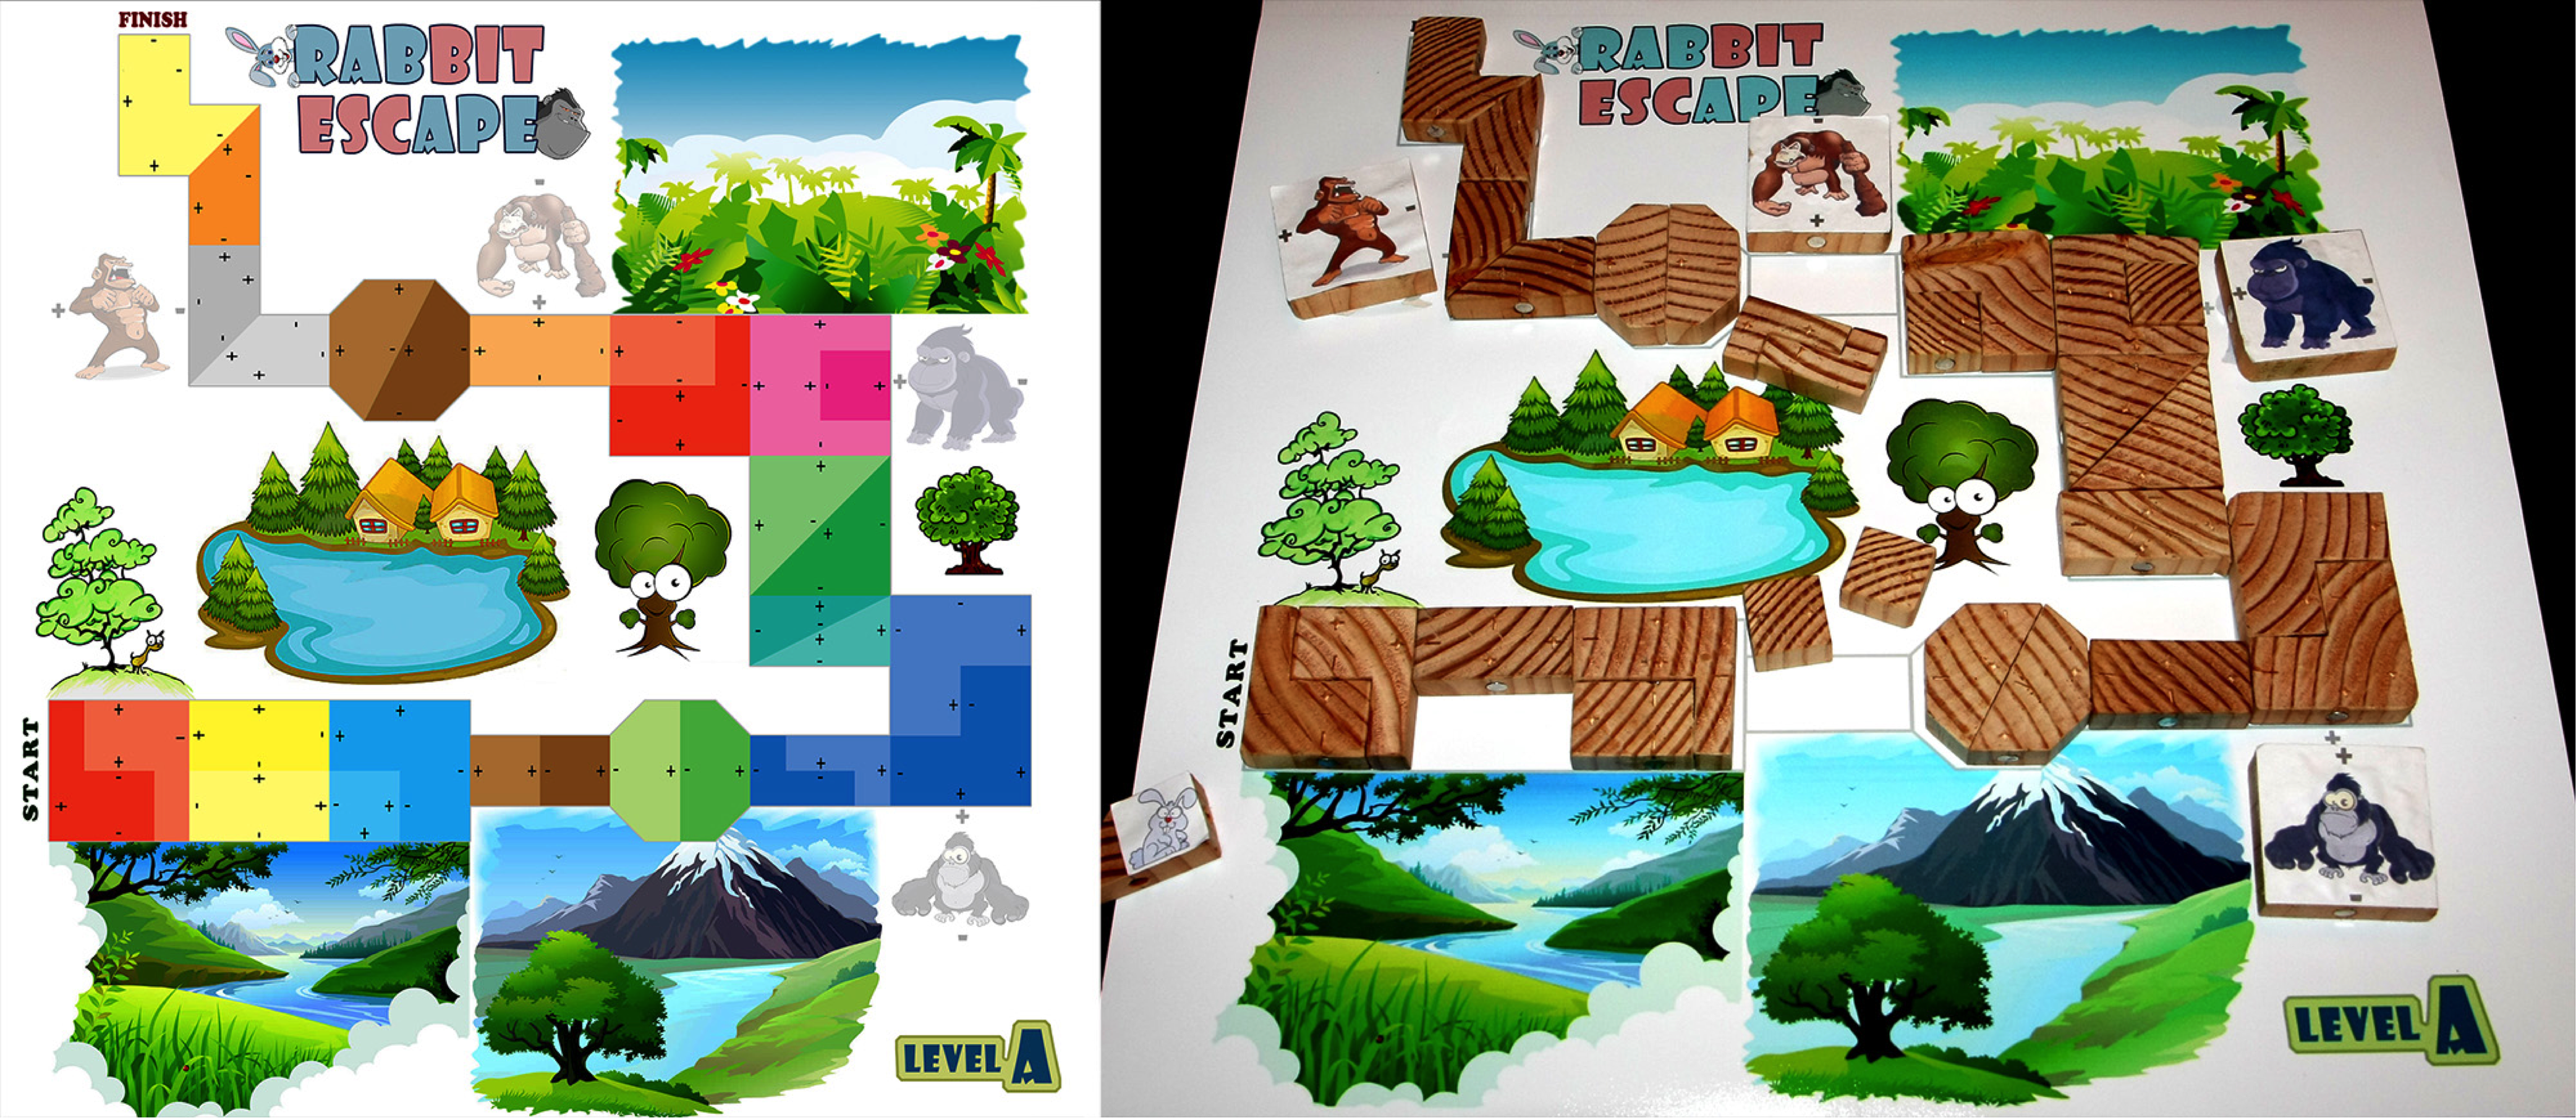
\includegraphics[width=0.48\textwidth]{boardgame.png}
  \caption{ (a) Designed completed board for first full level; (b) Physical game of the same board with most bits in place. }
  \label{fig:board-game}
\end{figure}

What makes the game especially challenging is the correct identification of the bits' properties and subsequent utilization of these properties to construct the blocks and then the whole path. These properties are:
\begin{itemize}
  \item{the size of each bit}
  \item{the position of the magnet on the bit}
  \item{the polarity of each magnet (engraved on the bit's long side)}
  \item{the orientation of the bit (or whole block)}
\end{itemize}

Players must combine all these attributes in order to put the bits next to each other in such a manner that they stick together at the right place (center or top of the bit's side), while also repelling the enemies positioned around the board.
Level A utilized all 29 pieces and all 4 enemies; we have made two variations, one with the block divisions drawn on the map and one without them.

\subsection{Play Strategies}
\label{sec:strategies}
% Training - Scaffolding
In order to help players understand the game mechanics and the importance of the different piece properties and how they affect completing the board effectively, we suggest a training session preceding the actual gameplay.
The session's purpose is to scaffold the players' understanding of how putting the pieces together allows them to construct different shapes and satisfy the activity objective. This need derived from our informal evaluation in a primary school and is described in more detail under the Instructional Design section.

The possible suggested activities for teaching CT with the game are described in more detail in the section that follows, although we understand that there are many variations that can derive from the suggested ones.

\subsubsection{Individual or Collaborative}
\label{sec:collaboration}
Players are given a predefined number of bits and a board and need to complete the board with all the pieces (i.e. build the path printed on the board), in a predefined amount of time (optional).
They are playing individually or as a team and can either place a block on the board in turns or negotiate about path building.
To increase difficulty they can add one or more of the enemy blocks by rolling the dice to decide enemy position; polarity is predefined on each board but players can reverse it to make the game easier or more difficult (preferably before starting the placement of the blocks).

Since each player has to conduct a rule-based plan based on their understanding of the game and combine their shared knowledge we consider this to be a manifestation of distributed computation.
Through the ``considerations, contingencies, and strategy formation'' of multiple parties a distributed cognition of different knowledge resources is created \cite{weller2008escape} and has to be maintained during the game to reach completion.
Distributed computation thinking was indicated as one of the distinguishing properties of CT compared to CS, according to the National Research Council \cite{national2010report}.

\subsubsection{Competitive}
\label{sec:competition}
Players are playing against each other and have to complete the path but starting from different directions.
They roll the dice and can place as many bits as the number rolled.
This activity demands well organized planning, since making the wrong choice will render the board impossible to complete.
The first student to complete the activity is the winner.
While advancing a longer path first may be considered making further progress, reaching a situation where there lack sufficient appropriate bits to complete the path results in the player having to disassemble the path to get the correct arrangement.
% Here we introduce a scoring system, but don't discuss points again later.
% Players get 1 point for every correct bit placed.
% They can change bits or blocks by deducting double the points of bits (e.g., 4 points for taking out 2 bits::1 block). 
% Taking off bits of the opponent's path is discouraged unless s/he consents, 
% in which case they both lose the exact number of points as the bits (e.g., 2 points each for taking out 2 bits).

This competitive mode demands efficient modeling skills since opponents would need to simulate the construction of a large portion of the board with the available pieces, to avoid the cost of losing points and negotiating retraction of a previous block or bit placement.
In a sense the effective combination of bit properties can be thought as algorithms that players need to compile during simulation in order to avoid these adverse consequences.
For example, deciding which two bits need to be placed together in a way to accommodate locking the blocks with adjacent ones (i.e., having the magnets in the right position and polarity), and do this for a series of blocks is a complex cognitive process similar to compiling an algorithm and testing hypothesis (simulation).
Both model building and simulation (forming and contrasting hypotheses) have been defined as foundational aspects of CT and revealed increased benefits compared to traditional methods of instruction \cite{wilensky2006thinking}.

\subsubsection{Board Construction}
\label{sec:construction}
With an entry point on one side of the board and finish on an exit point at another side, players can use all the bits or a random subset and make a custom path on an empty board.
They have to do this by drawing the blocks on the board but without placing the bits.
They will need to use the bits and blocks by creating a mental model of the path, taking each ``used'' block out before moving on, until they believe they have drawn the whole path.
Adding enemies would be optional to increase the difficulty of the game.
The second player (or another group of players) can then use this custom board to play the game in either of the first two ways.

Like the competitive activity, this construction method demands well organized planning to combine bit properties in order to make a playable board.
Considering bits and their properties to be the data, players need to construct sets of pieces as part of the path using logic during the process similarly to writing an algorithm (e.g. [conditional],``If I place this bit here, then this block has a minus on the bottom and needs a big square piece with a plus on the top center'').
This activity in particular demands the complex skill of combining different requirements to build a set of steps that will lead to an efficient solution to a problem (i.e., build a path from point \textit{A} to point \textit{B}, using \textit{X} number of pieces, and avoid \textit{Y} enemies) and has been defined as procedural thinking - teaching concept abstraction into algorithms \cite{papert1980mindstorms}, a core concept of CT \cite{national2010report}.

\subsection{Development of CT}
\label{sec:developing_ct}
RabBit EscApe satisfies most of the characteristics of the Operational Definition of CT for K-12 Education as defined by the International Society for Technology in Education (ISTE)\cite{operationalct}. 
More specifically, students playing the game should be able to: 1) logically organize and analyze data, 2) automate solutions through algorithmic thinking (a series of ordered steps), and 3) identify, analyze, and implement possible solutions with the goal of achieving the most efficient and effective combination of steps and resources. 
Considering the game mechanics and suggested activities discussed previously, we can make the following arguments considering support of these three characteristics:

\begin{enumerate}
\item{Bits have to be organized in blocks and block combinations that are meaningful according to bit properties and the printed path's form; pattern recognition is important in this process for identifying which bits create blocks that can fit the path printed on the board while also attracting adjacent blocks or repelling enemy blocks (demands analyzing the board based on possible bits combinations and organizing them on the path)}
\item{Board Construction setup demands that players devise some kind of strategy for correctly utilizing bits and matching the polarity and magnet position; for this purpose they need to come up with some kind of ``recipe'' for putting bits together while drawing the path on the board, also accounting for the remaining pieces (demands some kind of procedural or algorithmic thinking)}
\item{In all game setups, especially Individual/Collaborative and Competitive, players need to correctly identify the combination of blocks and bits by analyzing the path's comprising shapes and then simulate possible solutions for effectively completing the board, with the least number of bits and in the minimum time (efficiency).}
\end{enumerate}

XXXX Need to move the dispositions alongside the definition XXXX
Additionally, the game supports all dispositions and attitudes that are essential dimensions of CT, as expressed by the aforementioned definition which is pertinent to K-12 students:
\begin{itemize}
       \item \textbf{Confidence in dealing with complexity}:
       puzzles are inherently complex systems and without an operational strategy for dealing with complexity, the task might prove too challenging.
       RabBit EscApe introduces added complexity due to the additional puzzle piece properties that need to be accounted for.
       Confidence is built through successive iterations and attempts during the scaffolded activities, as discussed further under the section on Instructional Design.
       \item \textbf{Persistence in working with difficult problems}:
       deriving from the previous attitude, students are called to overcome initial frustration and persist in finding the solution. Our observations verified this point, since both teams finished the game with one wrong bit placement, but still persevered to start over and get the whole path completed correctly.
       \item \textbf{Tolerance for ambiguity}: 
       All three of the suggested play strategies include some degree of ambiguity deriving from either the complexity of the board and the amount of clues provided (e.g. including block divisions or a ``cheat sheet''), or from the collaborative or competitive nature of the game (i.e. no two  players have the same understanding about, nor expectations for the game). 
       \item \textbf{The ability to deal with open-ended problems}: Being able to cultivate the previous attitude naturally leads to practicing their ability to deal with open-ended problems. Game strategy C. Board Construction, especially, demands that players both have a good understanding of the game mechanics and bit properties, and are willing to deal with the messy process of modeling a new path with minimal constraints.
       \item \textbf{The ability to communicate and work with others to achieve a common goal or solution}:
       All three modes of play have been designed to encourage or demand some form of collaboration or competition.
       This requires players to externalize their mental models and rectify any misconceptions.
       Even in the competitive strategy, students have to express their intentions through negotiations with the opponent(s), as a means to achieve their individual or team goal.
\end{itemize}

\section{Evaluation and Observations}
\label{sec:observations}

We ran an informal pilot at an elementary school with two groups of three students each: one boy and two girls in each group, aged between 8 and 10 years. 
Both groups used the same board with play strategy A.Collaborative, but in one of them the dividers between blocks were not printed, making the game more open-ended and difficult. 
We followed Brandt's anecdote and interrogator method \cite{brandt1972studying} for data collection, to help protect the confidentiality of the students. More specifically, in order to protect our subjects' privacy, we took no notes, pictures, or videos during the actual session, but immediately thereafter wrote up the observations. 
Later in the same day, we interrogated each other's accounts and elaborated on the observations made, providing explanations whenever necessary. 
In addition to protecting the children's privacy, this method of data collection allowed us to devote our entire attention to observation, and not be distracted by documentation during the pilot.

The challenge of putting the puzzle together seemed relatively easy at first, as the students had many pieces available that could potentially fit within the path at any position. 
However we provided them with exactly as many pieces as they needed in our planned solution. 
The result was that once the students got good at placing the shapes within the lines, they had to confront the actual game challenges. 
They had to make sure that polarity was correct between the bits. Adjacent pieces should attract, rather than repel, each other, while pieces adjacent to the enemies should repel them. An additional challenge was found as they were trying to join the two ends of the path in the middle, since they started working at opposite ends (toward the middle) simultaneously. 
The result was a lucky scaling of difficulty/separation of concerns that was impossible to handle without a good understanding of the game mechanics.

At that point we decided to intervene by providing clues about the bit properties that children had to accommodate. 
In such an instance we tried to lead students in evaluating the different properties of a missing piece by themselves. 
Questions like, ``What does this big piece need to have?'' and, ``What do we know about it?'' while pointing at the larger block on the board (at the bottom right of {\em \hyperref[fig:board-game]{Figure \ref{fig:board-game}b}}) prompted students to use conditional logic (a fundamental concept of CT) in identifying the properties and eventually the piece. 
More specifically, one of the students started to respond to these prompts by saying, ``It is a big piece'' and then, ``it needs to have a plus magnet here'', while pointing at the bottom where the ape is, and ``it should have two more magnets on these sides,'' pointing at the top and bottom left where the large piece connects with the remaining path. 
Such instances indicated that students could grasp the conditions that had to be satisfied for successful block construction and placement.

We also noticed the way students communicated their intentions. 
At first, students described only the shape of the piece; however, they soon learned that the piece placement was too tightly constrained to merely try to swap out pieces of the same shape. 

After all, they could not be sure whether it was the piece in question that needed to be replaced, or its surroundings. 
They then realized that they should specify the shape and also the polarities of the magnets; however, even this was an underspecification. 
Because similarly shaped pieces may have the same number of magnets, but in different positions within a piece, they had to also specify the magnet locations. 
This demanded some kind of procedural or algorithmic thinking that is further discussed in the next section.

After almost 40 minutes of game play, both teams almost simultaneously thought they had completed the puzzle. 
At that point we encouraged the groups to compare their solutions. Each group discovered an error in the other team's solution as well as noting similarities and differences in their arrangements. 
Neither group had a solution that broke the lines of the path (so they satisfied this requirement); the errors discovered were single mistakes in polarity. 
Aside from their initial frustration, both teams demonstrated perseverance in starting over, despite the limited time remaining, and the fact that they basically had to start over again. This was an indication of willingness to confront the ambiguity in the game design.

Among many other interesting observations, there was a girl who seemed more systematic in bit placement. 
She was sometimes testing her hypotheses by pointing at the polarity signs while holding and rotating the bits in her hands, without actually trying to place them physically next to the ones on the board. 
This type of simulation is another important aspect of CT we have anticipated but have not systematically encouraged. 
Instances like this, but also the frustration caused by the lack of instructions and initial guidance, motivated us to consider the appropriate instructional interaction design that could help students play the game effectively while acquiring the largest learning benefits.

\section{\sloppy Instructional Interaction Design in support of Computational Thinking}
\label{sec:instructional_design}
Although we did not have sufficient time to complete a rigorous evaluation of RabBit EscApe, we discovered that scaffolding is a necessary step in enabling children to get the most out of such a game. 
Scaffolding includes levels of increasing difficulty, starting from making a single block (comprised of two to four bits) and moving on to more complicated shapes. 
At some points they will have the option to construct the different shapes using more than one combination of bits, and will have to incrementally take into account other piece properties and examine the implications of their choices. 
This mental modeling of the different affordances of each piece and the possible blocks it can construct will enable children to be more efficient in the actual game activities, without demanding extra cognitive load to process them during gameplay. 

Another idea to aid the bit selection and usage process is to have a separate ``cheat sheet'' with all pieces and their count, next to the actual game boards. 
Players can cross out any pieces that have been used with a marker in order to keep track of what has been used and what is still available. 
This cheat sheet can be used during the initial sessions where players are learning the available bits and practicing with the strategies of putting them together. 
Then, these mental aids can be progressively removed, letting the users depend on their ability to recognize the physical pieces. 
This is a common process of scaffolding in instructional design, also called fading, because the additional information (scaffold) is removed (faded) over time. 

These introductory puzzles can also assist in the pedagogical scaffolding necessary to promote CT and for the children to be able to complete more challenging puzzles by employing CT concepts. 
In order to deal with the underspecification problems that were observed during our pilot we suggest that children should have a very clear understanding of the piece properties and the constraints that they introduce. 
Thus, we need to help them form some kind of algorithmic representation including all the properties that bits should have in any given position, and show them how to apply it in similar situations. 
This can be achieved through guiding questions that will lead children to evaluate the different properties of any missing piece on the board. 
Questions like ``How big should this piece be?'', ``How should it attach to adjacent blocks?'', and ``What polarity should the magnets have?'' will help them construct mental functions of bit and path properties that need to be evaluated at every point in the game.

Social interactions are of pivotal importance in the conversion of the game attributes (i.e., path shape on board, bit properties, remaining bits) into mental functions. 
Students need not only rely on the guidance of a tutor but also on their peers; students should be encouraged to question each other's assumptions while moving from the initial introductory puzzles to more complex game boards. 
The goal would be to keep the students in the optimal cognitive state where they feel confident in dealing with the task at hand (i.e., forming parts of the path), but they are not overwhelmed by the complexity of the problem (i.e., completing the whole board). 
This condition, also known as the ``zone of proximal development'' \cite{vygotsky1987zone} is where learning is more effective, by internalizing external representations through social negotiations.

Finally, in designing this game for children, we recognize the importance of keeping the activity fun since this is a major motivating factor for children. 
Having colorful boards with a playful theme like the one used in the game (i.e., help the rabbit escape the lurking apes) is part of our instructional design approach that has been shown in our pilot to be effective, since children were compelled with the design and moved the rabbit piece even before fully completing the board. 
Teaching CT concepts in such a young age is not an easy task, thus we intentionally moved the focus of the game away from mathematical concepts which are predominant in similar game setups.

Through a sort of discovery process, we expect the children to use incremental formalism \cite{shipman1999formality} to indicate what pieces they are looking for, and simultaneously to enhance their spoken representation of the pieces. 
This may reflect evolution of their mental models of the game and its pieces as well. 

\subsection{Alternative Games Not Pursued}
\label{sec:terminated_games}
During our analysis of current games and brainstorming on new games that highlight teachable CT principles, two games also stood out alongside RabBit EscApe, a catapult game and a comic hero game.

The catapult game was a three stage game (interaction/ playground, test, and execute) where team members would learn how to operate a variable catapult to achieve desired results.
While the game design was quite concrete and well developed for addressing several CT principles not present in other games, consistent performance from the catapult at the scale we needed could not be achieved with the materials and size of the catapult chosen.
Another idea of a create-your-own superhero and enemy to compete against other characteristic specific heroes/enemies and student created heroes/enemies.
This game accentuates the creative nature of each student and challenges them in areas that align with more artistic definitions of CT, including modeling, 
The superhero game also offers opportunities to be one of the lowest cost games as it can involve just paper and a writing utensil similar to Live Action Role Playing games, where the imagination is paramount and requires descriptive well thought descriptions to be successful.

\subsection{Discussion}
\label{sec:discussion}
\sloppy Fabricating our own game was an interesting challenge.
Records must be established to keep track of which pieces have been cut, tapped, sanded, and implanted with magnets throughout the production stage.
The use of various custom jigs is important not only for speed, but also for consistent results require for peice alignment during gameplay.
For future work, we might propose just such exercises for high school students or above in a ``workshop''-style class.
% To determine the kind of physical and process scaffolding needed to produce consistent sizes of pieces in a timely fashion is important and difficult. 
From RabBit EscApe's theoretical design, we believe it shows promise for teaching CT. With additional levels that highlight common obstacles faced (ie. all pieces must have a southern faced )

\section{Conclusion}
\label{sec:conclusion}
\sloppy As CT continues to be discussed in academic and professional communities and until a more concrete definition emerges, a significant leap must be made to educate our communities' youth as society continues to develop computational systems with which they must interact, whether or not they can understand them. 

VT has embarked on a bold course to develop the CT capabilities of all its graduates.
Simultaneously the US National Science Foundation is funding research into how to develop these skills in the broader population.
While we think that VT can be effective in this pursuit, we believe that to truly change the CT of the population as a whole, we must have myriad interventions at various stages of an individual's formal and informal education.

In support of educating students at a younger age (than undergraduate students), we have developed RabBit EscApe to teach CT in a relatively explicit way.
We believe that addressing CT directly, in conjunction with more subtle interactions such as integrating CT with core content in existing formal education curricula \cite{NSFCE21} will best facilitate the learning of CT and its successful transfer and application to each individual's area of interest or expertise.

% We should discuss whether we should include text, annotations, or just y/n/m and switch to color coding. It appears we can fir everything in, but another run or look at it couldn't hurt, as we didn't do analysis on two of the games we listed
\clearpage
\begin{sidewaystable}[htbp]
\tiny
    \vspace*{-12cm}\hspace*{-1cm}\begin{tabular}{|p{1.5cm}||p{1.5cm}|p{2.5cm}|p{2.5cm}|p{2.7cm}|p{2cm}|p{1.5cm}|p{2cm}|p{3.5cm}|p{1.5cm}|}
    
    \hline

    Game
    & Modeling
    & Abstraction
    & Artistic Creation
    & Goal Disection
    & Risk/Reward == Comparison
    & Shared Roles
    & Patterns
    & Algortihms
    & Simulation \\ \hline \hline
    
    \multicolumn{10}{|l|}{Current Games}  \\ \hline \hline
    
    Pandemic
      & NO
      & NO
      & NO 
      & \cellcolor{blue!25}YES 
      & \cellcolor{blue!25}YES 
      & \cellcolor{blue!25}YES 
      & \cellcolor{blue!25}YES 
      & NO 
      & NO \\ \hline
    
    Settlers Of Catan 
      & NO 
      & NO 
      & NO 
      & \cellcolor{blue!25}YES 
      & NO 
      & NO 
      & NO 
      & NO 
      & NO \\ \hline

    Robot Turtles 
      & NO 
      & NO 
      & NO 
      & \cellcolor{blue!25}YES 
      & NO 
      & NO 
      & \cellcolor{blue!25}YES 
      & \cellcolor{blue!25}YES 
      & \cellcolor{blue!25}YES \\ \hline

    Mr. Jack 
      & NO 
      & NO 
      & NO 
      & \cellcolor{blue!25}YES 
      & NO 
      & NO 
      & NO 
      & NO 
      & NO \\ \hline

    Ticket To Ride 
      & NO 
      & NO 
      & NO 
      & \cellcolor{blue!25}YES 
      & NO 
      & NO 
      & \cellcolor{blue!25}YES 
      & NO 
      & NO \\ \hline

    Carcassonne 
      & NO 
      & NO 
      & NO 
      & \cellcolor{blue!25}YES 
      & NO 
      & NO 
      & NO 
      & NO 
      & NO \\ \hline

    Guess Who 
      & \cellcolor{blue!25}YES 
      & NO 
      & \cellcolor{blue!25}YES 
      & \cellcolor{blue!25}YES 
      & NO 
      & NO 
      & \cellcolor{blue!25}YES 
      & \cellcolor{blue!25}YES 
      & NO \\ \hline

    Chess 
      & In formations 
      & NO 
      & NO 
      & MAYBE 
      & NO 
      & NO 
      & NO 
      & \cellcolor{blue!25}YES, but even strong computers fail at this 
      & NO \\ \hline

    Checkers 
      & NO 
      & NO 
      & NO 
      & NO 
      & \cellcolor{blue!25}YES 
      & NO 
      & NO 
      & NO 
      & NO \\ \hline

    Blockus 
      & NO 
      & NO 
      & NO 
      & \cellcolor{blue!25}YES 
      & NO 
      & NO 
      & \cellcolor{blue!25}YES 
      & \cellcolor{blue!25}YES, in end game 
      & NO \\ \hline

    % Resistance 
    %   & NO 
    %   & NO 
    %   & NO 
    %   & NO 
    %   & NO 
    %   & NO 
    %   & NO 
    %   & NO 
    %   & NO 
    %   & NO \\ \hline

    Acquire 
      & NO 
      & NO 
      & NO 
      & \cellcolor{blue!25}YES 
      & NO 
      & NO 
      & NO 
      & NO 
      & NO \\ \hline

    Tic Tac Toe
      & NO 
      & NO 
      & NO 
      & NO 
      & NO 
      & NO 
      & \cellcolor{blue!25}YES 
      & \cellcolor{blue!25}YES 
      & NO \\ \hline

    Clue
      & NO 
      & NO 
      & NO 
      & NO 
      & \cellcolor{blue!25}YES 
      & NO 
      & NO 
      & \cellcolor{blue!25}YES 
      & NO \\ \hline

    3-15
      & NO 
      & NO 
      & NO 
      & \cellcolor{blue!25}YES 
      & NO 
      & NO 
      & NO 
      & NO 
      & NO \\ \hline

    Cranium
      & NO 
      & NO 
      & \cellcolor{blue!25}YES 
      & NO 
      & NO 
      & \cellcolor{blue!25}YES 
      & NO 
      & NO 
      & NO \\ \hline

    Battleship 
      & NO 
      & \cellcolor{blue!25}YES 
      & NO 
      & NO 
      & NO 
      & NO 
      & \cellcolor{blue!25}YES 
      & \cellcolor{blue!25}YES 
      & NO \\ \hline

    Dominoes 
      & NO 
      & NO 
      & NO 
      & NO 
      & NO 
      & NO 
      & NO 
      & \cellcolor{blue!25}YES 
      & NO \\ \hline

    Mad Lib 
      & \cellcolor{blue!25}YES 
      & NO 
      & \cellcolor{blue!25}YES 
      & NO 
      & NO 
      & NO 
      & NO 
      & NO 
      & NO \\ \hline \hline    

    \multicolumn{10}{|l|}{Proposed Games} \\ \hline \hline

    nMotion (Catapult)
      & \raggedright{Weapons, targets, ammunition, play field (with constraints)} 
      & \raggedright{Methods vs models, Trial \& error to understand each model.\newline \newline The different stages (play|design|test) allow for stronger abstractions, especially across situations} 
    % & \raggedright{EASY: Aim, prime, fire, and move.\newline \newline DIFFICULT: switch people, defend, and how to define communication(parameters) to each other} 
      & \raggedright{Less so, but maybe if they create their own weapon from methods/functions.\newline \newline Or are allowed to create a defense} 
      & \raggedright{Starting with a goal, they identify the components that will help them achieve their goal.
        Several layers of dissection will need to occur to be proficient} 
      & \raggedright{Given a limited number of attempts}     
      % & \raggedright{A correct analysis of the situation, as well as appropriate selection and execution of methods enables role playing and challenges that should expand stronger methods, models, and artistic creation.} 
      & \raggedright{Team based competition} 
      & \raggedright{There are patterns in the trial and error in recognizing performance} 
      & \raggedright{The students can create a set of nested steps to perform tasks.\newline \newline The effectiveness of another team member executing the task without any follow up communication (verbal or other) can be measured.
        The team's collective algorithms could be assessed on another team performing the task and the questions that arise out of their performance.} 
      & {\raggedright The play phase of this game is simulation} \\ \hline
    
    Hero Game 
      & \cellcolor{blue!25}YES 
      & \cellcolor{blue!25}YES 
      & \cellcolor{blue!25}YES 
      & NO 
      & \cellcolor{blue!25}YES 
      & NO 
      & NO 
      & NO 
      & NO \\ \hline
    
    Sorting height of students 
      & NO 
      & NO 
      & NO 
      & \cellcolor{blue!25}YES 
      & NO 
      & NO 
      & NO 
      & \cellcolor{blue!25}YES 
      & NO \\ \hline
    
    % Collaborative matching 
      % & NO 
      % & NO 
      % & NO 
      % & NO 
      % & NO 
      % & NO 
      % & NO 
      % & NO 
      % & NO \\ \hline
    
    Mixing water Bottles (from Die Hard \cite{diehard2008thorp}) 
      & \cellcolor{blue!25}YES 
      & \cellcolor{blue!25}YES 
      & NO 
      & \cellcolor{blue!25}YES 
      & NO 
      & NO 
      & \cellcolor{blue!25}YES 
      & NO 
      & NO \\ \hline
    
    Bi Directional Mad Libs 
      & \cellcolor{blue!25}YES 
      & \cellcolor{blue!25}YES 
      & \cellcolor{blue!25}YES 
      & NO 
      & NO 
      & NO 
      & NO 
      & NO 
      & NO \\ \hline
    
    Rab-Bit Esc-Ape 
      & \raggedright{The wooden bits and designated path structures} 
      & NO 
      & \raggedright{Creating new path levels} 
      & \raggedright{Path must be broken down into chunks and separate models constructed for each chunk} 
      & \raggedright{Given a time restriction, strategies come into play} 
      & \raggedright{Players can choose to work either in different parts of the board or the same one} 
      & \raggedright{Bit combinations, by analyzing the path, the enemies, and magnet polarity}
      & \raggedright{reusability of paths or components across game boards; extra points are awarded for using such blocks.
        Over time they get better at this `algorithmic' approach of reusing bits per case (e.g., round corners, U turns, etc.)} 
      & NO \\ \hline

    \end{tabular}\hspace*{-1cm}\vspace*{-1cm}
    \hspace*{1cm}\vspace*{1cm}\caption{Comparison of Games}
    \label{table:games-comparison}
\end{sidewaystable}

\clearpage
%ACKNOWLEDGMENTS are optional
% \section{Acknowledgments}
% Dane Webster, our CT class?

%
% The following two commands are all you need in the
% initial runs of your .tex file to
% produce the bibliography for the citations in your paper.
\bibliographystyle{abbrv}
% \bibliography{sigproc} % sigproc.bib is the name of the Bibliography in this case
% You must have a proper ".bib" file
% and remember to run:
% latex bibtex latex latex
% to resolve all references
%
% ACM needs 'a single self-contained file'!
%
%APPENDICES are optional
%\balancecolumns
% \appendix
% %Appendix A
% \section{Headings in Appendices}
% The rules about hierarchical headings discussed above for
% the body of the article are different in the appendices.
% In the \textbf{appendix} environment, the command
% \textbf{section} is used to
% indicate the start of each Appendix, with alphabetic order
% designation (i.e. the first is A, the second B, etc.) and
% a title (if you include one). So, if you need
% hierarchical structure
% \textit{within} an Appendix, start with \textbf{subsection} as the
% highest level. Here is an outline of the body of this
% document in Appendix-appropriate form:
% \subsection{Introduction}
% \subsection{The Body of the Paper}
% \subsubsection{Type Changes and Special Characters}
% \subsubsection{Math Equations}
% \paragraph{Inline (In-text) Equations}
% \paragraph{Display Equations}
% \subsubsection{Citations}
% \subsubsection{Tables}
% \subsubsection{Figures}
% \subsubsection{Theorem-like Constructs}
% \subsubsection*{A Caveat for the \TeX\ Expert}
% \subsection{Conclusions}
% \subsection{Acknowledgments}
% \subsection{Additional Authors}
% This section is inserted by \LaTeX; you do not insert it.
% You just add the names and information in the
% \texttt{{\char'134}additionalauthors} command at the start
% of the document.
% \subsection{References}
\bibliography{sigproc}
% Generated by bibtex from your ~.bib file. Run latex,
% then bibtex, then latex twice (to resolve references)
% to create the ~.bbl file. Insert that ~.bbl file into
% the .tex source file and comment out
% the command \texttt{{\char'134}thebibliography}.
% This next section command marks the start of
% Appendix B, and does not continue the present hierarchy
% \section{More Help for the Hardy}
% The acm\_proc\_article-sp document class file itself is chock-full of succinct
% and helpful comments. If you consider yourself a moderately
% experienced to expert user of \LaTeX, you may find reading
% it useful but please remember not to change it.
\balancecolumns
% That's all folks!
\end{document}
